\chapter{凸分析}\label{chap:convex-analysis}

你上山采过蘑菇吗?尽管蘑菇是一种美味的食材,但是市场上迟到的大部分蘑菇都是人工养殖的. 在中国云南,一片神奇的土地上,当地人非常喜欢食用野生生长的蘑菇,俗称“野生菌”. 比起人工养殖的蘑菇,野生菌的风味要丰富和鲜美得多. 

在一众野生菌中,一种叫“松茸”的种类最为珍惜名贵,松茸因其产量少、价值高而显得极其珍贵,被誉为“万菌之王”. 迄今为止,松茸在世界上尚不能进行真正意义上的纯人工栽培,并且大多生长在高山林中,只能依靠人工寻找采摘. 

如果让你上山去采松茸,但你对松茸一无所知,你会怎么做?你只能一点一点地摸索,爬遍整座山,对这图鉴寻找和它匹配的野生菌. 这个过程非常耗时耗力,而且大概率无功而返. 实际上,松茸价格昂贵就是因为它的稀有性. 

然而,如果有一个向导,非常熟悉这些山,年年采摘松茸,虽然他也不知道松茸的确切位置,但是他可以凭借经验,大幅减少寻找的范围和时间. 因此,在向导的帮助下,你采摘的成功率和效率都会很大提高. 

乍一看,找松茸的故事也许与AI没有关系. 然而,我们在现实中面对的很多问题都是在找松茸:我们希望找到一个预测准确率最高的机器学习模型、一个最优的分配方案、一条最快的导航路线等等. 这些问题都是本质上都是决策与优化的问题. 

我们自然希望可以高效地求解这些问题,但是,正如松茸的稀缺性,我们希望找到的东西往往是“稀有”的. 如果我们对问题的结构一无所知,我们只能非常低效地进行搜索,这就好比我们在山上摸索寻找松茸. 然而,如果我们对问题的结构有所了解,我们就可以像拥有向导一样,利用这些信息来指导我们的搜索,从而提高效率. 

本章将会建立关于决策与优化的基本理论,并指出其中一种极其重要的特例:\emph{凸优化},这是一类存在良好结构的优化问题,因而可以被高效求解. 特别地,凸优化关心的对象被称为\emph{凸函数}和\emph{凸集},我们将初步探究凸函数和凸集的性质. 

\section{决策与优化的基本原理}\label{sec:decision-optimization-principle}

首先,我们介绍决策与优化的基本原理. 我们会从统计决策理论出发,然后讨论优化是什么,在做什么,有什么最基本的事实. 

\subsection{统计决策理论}

我们考虑一个最简单的情形,统计中国大学生的平均身高. 2023年,中国在校大学生有4700多万人,我们自然很难真的去测量每一个人的身高,然后算一个平均值. 因此,我们只能通过抽样的方式来估计这个平均值. 

我们抽取了1000名大学生,测量他们的身高,然后计算这1000名大学生的平均身高. 这个平均身高就是我们的\emph{统计决策},我们的目标是希望这个平均身高能够尽可能地接近真实的平均身高. 

上面简单的例子其实具有一般性. 在\Cref{chap:information-theory}我们讨论过,我们可以从一堆对象中提取信息. 我们把我们所关心的集合对象称为(随机)\emph{总体} $P$. 从概率论角度看,总体就是一个概率分布. 现在我们从总体$P$中抽取一个\emph{样本} $X$. 这件事情在概率论上意味着我们得到了一个随机变量$X$服从分布$P$. 

拿到样本之后,我们的任务是做出\emph{好的决策}.
\begin{itemize}
    \item 决策$T$是一个依赖$X$的函数. 比如说,$P$是所有大学生的身高,$X$是随机抽选一个人测量的身高,我们的决策$T$是估计大学生的平均身高.\footnote{注意,这里我们说的只是抽选一个人测量的身高,而不是抽取1000人的身高. 如果要适配本节开头的例子,那么总体是1000个大学生身高的分布,而样本是1000个大学生的身高. }
    \item “好的决策”指的是函数$T$能够具备某些量化指标. 其中非常常用的一个方法是通过\emph{损失函数}来衡量,它是总体$P$和决策$T(X)$的函数,即$L(P,T(X))$. 例如,我们可以用
    \[L(P,T(X))=|\E_{X\sim P}[X]-T(X)|\]
    来衡量估计的平均身高和真实平均身高的差距.
\end{itemize}

\begin{remark}
    损失函数在不同语境下有不同称呼. \emph{损失函数}是机器学习和数理统计语境下常用的称呼. 在控制理论中以及机器学习中,它被称为\emph{代价函数}. 在经济学和金融学的风险理论中,损失函数被称为\emph{风险函数},它意味着个体在面对不确定的环境下所需要面对的风险. 而在优化理论中,损失函数往往被称为\emph{目标函数},表明所要优化的对象. 
\end{remark}

决策$T$的一种量化指标是最小化期望意义下的损失函数:
    \[\min_{T}\E_{X\sim P}[L(P,T(X))].\]
在经济学中,这一量化指标实际上是von Neumann和Morgenstern \emph{期望效用理论}的具体体现,我们会在\Cref{sec:mixed-strategy}中详细讨论. 这一理论认为,个体在面对不确定的环境时,会选择最大化期望效用的决策;在这里,就是最小化期望损失的决策.

现在我们考虑一个非常一般的决策任务. 假设我们的任务是估计函数$f$,但是我们只知道观测到的自变量$X$(来自总体$P$)以及它的函数值$Y=f(X)$,我们的决策是函数的估计值$\hat f$. 在机器学习中,$f$通常是需要训练的模型. 我们可以写出若干种损失函数:
\begin{itemize}
    \item 平方($L^2$)损失函数:$L(P,T(X))=(Y-\hat f(X))^2$. 使用此损失函数的时候,我们要假定$f$在实数范围取值. 
    \item $L^1$损失函数:$L(P,T(X))=|Y-\hat f(X)|$. 使用此损失函数的时候,我们要假定$f$在实数范围取值. 
    \item SVM损失函数(hinge损失函数):$L(P,T(X))=\max\{0,1-Y\cdot\hat f(X)\}$. 使用此损失函数的时候,我们一般要假定$f(X)\in[-1,1]$. 
    \item 交叉熵损失函数:$L(P,T(X))=CH(\hat f(X),Y)$. 在二分类问题中,我们假设$Y$的取值为$0$或$1$,分别代表负类和正类. 函数的估计值$\hat f (X)$输出的是样本$X$属于正类的概率,而我们把$Y$看成退化分布,此时交叉熵损失函数衡量的是$\hat f(X)$和$Y$之间的差距.
\end{itemize}

通常,我们不能知道总体$P$的分布是什么,只知道样本$X_1,\dots,X_n$,此时我们用平均损失来代替期望损失:
    \[\min_{T}\frac{1}{n}\sum_{i=1}^n L(P,T(X_i)).\]

这些损失函数会用在不同的场景之中. 通常来说,机器学习中有两类问题:\emph{回归问题}和\emph{分类问题}. 他们两个的区别主要在于:
\begin{itemize}
    \item 回归问题中,$f$取值为实数,而且通常随自变量连续变化;而分类问题中,$f$只取有限多个值,他们通常被作为标签(比如这张图片是人还是青蛙)使用.
    \item 在回归问题中,我们通常使用平方损失函数或者$L^1$损失函数;在分类问题中,我们通常使用SVM损失函数或者交叉熵损失函数.
\end{itemize}

\subsection{优化问题}
现在我们从决策过渡到优化. 在最简单的决策问题中,我们的目标就是找到某个$x$使得(期望)损失函数$f$最小. 此时,问题的一般形式为:
\begin{equation}
\begin{alignedat}{2}
\min_{x}&\quad f(x)\\
\text{s.t.}&\quad f_i(x)=0,&\quad i=1,\dots,m,\\
&\quad g_j(x)\leq 0,&\quad j=1,\dots,n,\\
&\quad x\in\Omega.
\end{alignedat}
\label{eq:opt-general}
\end{equation}
这里,s.t(subject to)之后的内容表明了$x$取值的限制,因此被称为\emph{约束}. 其中$f_i(x)=0$和$g_j(x)\leq 0$被称为\emph{函数约束},而$x\in\Omega$被称为\emph{集合约束}.

通常,为了简化记号,我们会把函数约束用向量的形式表示,比如,用
\begin{align*}
    &f(x)=0,\\
    &g(x)\leq 0.
\end{align*}
来表示 \eqref{eq:opt-general} 中的函数约束. 

如果和本章开头的故事对比,能最小化$f$的那个$x$就是我们要找的松茸,而我们要爬的山就是 \eqref{eq:opt-general}. 不同的山自然有不同的特性,在优化这里,根据损失函数$f$、约束条件$f_i$和$g_j$的不同性质,我们可以对优化问题进行分类:
\begin{itemize}
\item 无约束优化:约束条件$f_i$和$g_j$实际上不存在,即$m=n=0$,并且$\Omega$是全空间,比如$\R^n$.
\item 有约束优化:至少存在一个约束条件,即$\min\{m,n\}\geq 1$,或者$\Omega$不是全空间. 
\item 光滑优化:损失函数和约束条件都是可微函数.\footnote{光滑这一词的含义在不同的文献中大相径庭,它可以指(连续)可微、连续可微、二次(连续)可微或者无穷次可微. }
\item 线性优化:损失函数和约束条件都是线性函数(形如$a^\t x+b$).
\end{itemize}

如此纷繁的分类,实际上是为了更好地理解优化问题的性质. 不同的特殊结构会给优化带来特殊的性质,从而可以设计出更高效的算法.

下面我们看几个经典的优化例子. 
\begin{example}[最小二乘法]\label{ex:least-square}
    给定矩阵$A\in\R^{m\times n}$和向量$b\in\R^m$,考虑如下优化问题:
    \begin{alignat*}{2}
    \min_{x}&\quad \norm{Ax-b}_2^2\\
    \text{s.t.}&\quad x\in\R^n.
    \end{alignat*}
    这个问题被称为\textbf{最小二乘法}. 目标函数可以被写为$(Ax-b)^\t(Ax-b)$,因此最小二乘法是一种典型的无约束光滑优化问题. 

    最小二乘法的解$x^*$实际上是\emph{投影}解. 为了说明这一点,我们需要基本的线性代数知识,请参阅\Cref{chap:linear-algebra}. 
    
    具体来说,我们把$Ax$理解为$A$的列向量的线性组合,于是整个优化问题可以被看成找一个向量到某个线性空间的最短距离,即投影,如\Cref{fig:projecting} 所示. 
    \begin{figure}[H]
    \centering
    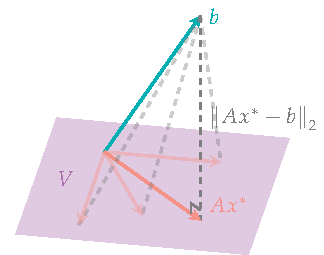
\includegraphics[width=0.6\textwidth]{Figures/convex-anlaysis/projecting.pdf}
    \caption{最小二乘法的几何解法}\label{fig:projecting}
    \end{figure}

    我们现在从代数上解释这张图. 我们可以得到一个线性子空间
    \[V=\{Ax:x\in\R^n\}.\]
    全空间$\R^m$可以被分解为两个正交的子空间$V$和$V^\perp$,其中$V^\perp$是$V$的正交补:
    \[\R^m=V\oplus V^\perp.\]
    于是,$b$可以被分解为$V$和$V^\perp$的分量:
    \[b=b_V+b_{V^\perp}.\]
    其中$b_V$可以被写作某个$Ax^*$. 
    
    因此,优化的目标可以重新写作
    \begin{align*}
        \norm{Ax-b}_2^2&=\norm{Ax-b_V-b_{V^\perp}}_2^2\\
        &=\norm{Ax-b_V}_2^2+\norm{b_{V^\perp}}_2^2\\
        &=\norm{A(x-x^*)}_2^2+\norm{b_{V^\perp}}_2^2.
    \end{align*}
    当$x=x^*$时这一目标函数取到最小值. 
    
    因此,我们利用特殊的几何结构,可以把最小二乘法转化为一个投影问题,从而高效求解. 反之,求投影也可以被写作一个优化问题. 
\end{example}

\begin{example}[线性规划]\label{ex:linear-programming}
    给定矩阵$A\in\R^{m\times n}$和向量$b\in\R^m$,考虑如下优化问题:
    \begin{alignat*}{2}
    \min_{x}&\quad c^\t x\\
    \text{s.t.}&\quad Ax\leq b,\\
    &\quad x\geq 0.
    \end{alignat*}
    这个问题被称为\textbf{线性规划}. 目标函数和约束条件都是线性的,因此线性规划是一种典型的线性优化问题. 注意,我们上面已经用了向量不等式的函数约束形式. 
\end{example}

上面两个例子远远不能覆盖所有的优化问题,实际上,相当多的运筹学、机器学习和计算机科学中的问题都可以被视作(非线性)优化问题. 
\begin{itemize}
    \item 运筹学:线性规划、二次规划、整数规划、网络流问题、组合优化问题等.
    \item 金融学:投资组合优化、风险控制等.
    \item 机器学习:模型的训练.
    \item 计算机科学:图论中的极值问题,例如最短路径问题、最小生成树问题等.
\end{itemize}

如果有能够解决一般优化问题的灵丹妙药,那么将会有极其重大的意义. 然而我们后面将会看到,一般的优化是一个难解的问题,更严谨一点说,\emph{不存在通用高效算法}. 

我们先需要明确什么是\emph{优化算法},它应该要具备如下特征:
\begin{itemize}
    \item 大部分优化算法都用了\textbf{迭代法}的思想:算法$A$接受一个自变量$x$,输出一个自变量$A(x)$,并把它作为下一轮的输入.
    \item 此外,一个算法还应该具有\textbf{通用性},即它必须要能解决一类优化问题$F$.
    \item 然后,算法具备通用性就意味着它在进行\textbf{黑箱优化}:$F$必须要给算法提供必要的信息来完成求解,我们将这样的提供机制抽象为\textbf{先知},记为$\O$. 具体来说算法输入$x$给$\O$,$\O$返回一些信息给算法(例如$x$处的函数值、导数值、Hessian矩阵).
\end{itemize}

接下来的问题是衡量优化算法的性能好坏. 我们关注的是\emph{最坏情况},也就是说假如我们关注的是问题类$P\subseteq F$,那么,我们要看的是优化算法在$P$中最差的表现如何. 衡量优化算法性能的指标有以下几个:

\begin{itemize}
    \item \textbf{近似程度}:我们需要求在允许误差$\epsilon$的情况下的近似解. 例如,函数值不大于最优值的$\epsilon$,或者离最优点距离不超过$\epsilon$. 考虑近似解是优化问题非常重要的一个想法,因为计算机的表示精度是有限的,我们不可能在所有情况下都求出精确解,所以求近似解是合理的要求. 
    \item \textbf{运行时间}(\textbf{收敛速度},\textbf{复杂度}):找到目标近似解需要调用先知的次数. 通常来说,运行时间会随近似度要求变高而变长,因此运行时间是一个关于近似程度的函数.
\end{itemize}

\begin{remark}
    通常来说,优化算法的执行过程中还会进行除了调用先知之外的操作,例如进行加减乘除. 然而,如果我们把所有这些操作都算入复杂度之中,算法的分析会变得非常困难,因此我们通常只考虑调用先知的次数. 
    
    这样做的合理性在于,每一次的加减乘除等额外操作,几乎都是因为调用一次先知所以才进行的,因此我们可以把这些额外操作的时间都算入先知调用的时间之中. 
\end{remark}

为了陈述“没有万能算法”这一事实,我们还需要引入一些记号. 

设$F$是有限个优化问题的集合,优化的可行域是有限集,目标函数的到达域也是有限集,$F$上有一个任意的概率分布.\footnote{例如考虑64位浮点数,此时,尽管可行域和目标函数的到达域非常庞大,但都是有限集.}

记号$d_t$表示$t$轮迭代之后算法产生的点列
\[(x_t(1),y_t(1)),\dots,(x_t(t),y_t(t)).\]
其中$x_t(k)$是算法在第$k$轮迭代中产生的点,$y_t(k)$是这一步的函数值.

给定迭代轮数$t$,优化问题$f$,算法$A$,优化过程所产生的点列概率分布为
\[P(d_t|f,t,A).\]

有了上面这些记号,我们就可以将“没有万能算法”这一陈述写成定理了. 

\begin{theorem}[没有免费午餐定理]\label{thm:no-free-lunch}
对任意优化算法$A_1,A_2$,
    \[\sum_{f\in F} P(d_t|f,t,A_1)=\sum_{f\in F} P(d_t|f,t,A_2).\]
\end{theorem}

这一定理的证明可以用归纳法实现,我们将它留作习题(见习题\lhysays{出一下}).

没有免费午餐定理意味着,对特定的点列,任何算法在所有实例上产生它的概率总和是一样的. 

那么,点列和“没有万能算法”有什么样的关系呢?实际上,衡量算法性能的指标和点列有非常密切的联系. 比如说,算法花了$k$步找到一个$\epsilon$-近似解,用点列的语言来说就是,算法迭代产生的点列,长度至多是$k$并且最后一个点距离最优解距离不大于$\epsilon$. 

更一般地,算法具有某种指标的性能,就意味着算法可以产生某些特定的点列. 因此,对于任何一类优化问题来说,不论以何种指标来衡量性能,优化算法在某些问题上表现出来的突出性能一定会在另一些问题上被抵消. 没有一个万能的算法可以高效解决所有优化问题!

\begin{remark}
    在现实中,真的没有免费午餐吗?注意,没有免费午餐定理所谓的性能抵消,是条件在$f$意义上的. 但是,如果我们将$f$本身的先验概率分布也纳入考虑,那么有一些算法平均的性能可能会更好.(回忆\Cref{chap:plausible-reasoning}中的基率谬误与Simpson悖论)
    
    在现实生活中,我们需要求解的优化问题都是天然有某种先验分布的,因此我们可以利用这个信息来设计更好的算法. 这同样遵循着优化的基本原理:如果我们可以利用问题的结构,那么我们就可以更高效地求解问题.
\end{remark}

\subsection{例子:网格搜索算法}

前面对于概念的讨论可能比较抽象,所以下面我们看一个具体的例子,这个例子将会展示从算法分析的角度,优化所关注的主要问题. 考虑如下优化问题:
\begin{equation}
    \begin{aligned}
    \min_{x}&\quad f(x)\\
    \text{s.t.}&\quad x\in[0,1]^n.
\end{aligned}\label{opt:grid-search}
\end{equation}
其中$f(x)$是Lipschitz连续函数,即它满足
    \[|f(x)-f(y)|\leq L\norm{x-y}_\infty,\quad\forall x,y\in[0,1]^n.\]
关于优化算法的假设如下. 首先,我们可以访问\textbf{零阶先知},即$\O(x)=f(x)$. 其次,优化算法需要去找到\textbf{$\epsilon$-近似解},即函数值至多比最小值大$\epsilon$的解.

\begin{remark}

        在优化中,我们会经常使用词语“零阶”“一阶”等等,所谓的“阶”指的是函数导数阶数,零阶先知指的是我们可以访问函数值,一阶先知指的是我们可以访问一阶导数,以此类推. 后面还会有零阶条件、一阶条件等等,他们的含义类似. 
\end{remark}

我们考虑一个非常简单的算法,它被称为\emph{网格搜索}:
\begin{itemize}
    \item 将$[0,1]$等分成$p$份,$[0,1]=[0,1/p]\cup\dots[(p-1)/p,1]$.
    \item 遍历$(p+1)^n$个格点:
    \[x_{(i_1,\dots,i_n)}=\left(\frac{i_1}{p},\dots,\frac{i_n}{p}\right)^\t,\]
    $i_k\in\{0,1,\dots,p\}$.
    \item 对每个格点询问先知得到其函数值,输出函数值最小的一个(记为$(\bar{x},f(\bar x))$).
\end{itemize}

这一算法和我们在山上找松茸的故事有异曲同工之妙:我们爬山找松茸的时候,也是将整座山分成很多小块,然后在每个小块上找松茸,最后找到最好的那个.

我们对于网格搜索算法问的问题是,它的复杂度如何. 也就是说,它需要调用先知多少次才能找到一个$\epsilon$-近似解?我们从一个引理开始. 

\begin{lemma}\label{lemma:grid-search}
    设 \eqref{opt:grid-search} 的最优值为$f^*$,那么
\[f(\bar x)-f^*\leq\frac{L}{2p}.\]
\end{lemma}
\begin{proof}
设$x^*$是最优点,存在一个方格包含$x^*$:
\[x_{(i_1,\dots,i_n)}\leq x^*\leq x_{(i_1+1,\dots,i_n+1)}.\]
这个方格的长为$1/p$,所以我们可以选取方格的某个顶点$\hat x$,使得它的每一个轴离$x^*$的距离都不超过$1/(2p)$,如\Cref{fig:grid-partition} 所示. 

\begin{figure}[H]
    \centering
    \lhysays{画个图}
    \caption{网格示意图}
    \label{fig:grid-partition}
\end{figure}

于是根据Lipschitz条件,
    \[f(\bar x)-f^*\leq f(\hat x)-f(x^*)\leq L\norm{\hat x- x^*}_\infty\leq \frac{L}{2p}.\]
\end{proof}

利用这个引理,我们可以证明网格搜索算法的复杂度.
\begin{theorem}
    网格搜索算法可以找到找到一个$\epsilon$-近似解,其调用$\O$的次数至多为
    \[\left(\left\lfloor\frac{L}{2\epsilon}\right\rfloor+2\right)^n.\]
\end{theorem}
\begin{proof}
    取$p=\lfloor L/(2\epsilon)\rfloor+1$,代入\Cref{lemma:grid-search} 即可.
\end{proof}

网格搜索法的运行时间给了优化问题 \eqref{opt:grid-search} 一个求解时间的\textbf{上界}. 然而这个上界和维数呈指数关系,通常来说都是不可接受的复杂度. 

自然地,我们会问,\eqref{opt:grid-search} 会有更好的算法吗? 这就是\textbf{下界问题}. 令人惊讶的是,对于这一个问题,我们可以证明网格搜索法是渐近意义下最优的!

\begin{theorem}\label{thm:grid-search-lower-bound}
    设$\epsilon<L/2$,要想对任意$f$都能找到 \eqref{opt:grid-search} 的 $\epsilon$-近似解,访问$\O$的算法(零阶算法)找到至少需要调用$\O$
    \[\left\lfloor\frac{L}{2\epsilon}\right\rfloor^n\]
    次.
\end{theorem}
\begin{proof}
设$p=\lfloor L/(2\epsilon)\rfloor$,对任意算法$A$,我们尝试构造一个函数,使得$A$调用$\O$的次数小于$p^n$时最多找到一个$\epsilon$-近似解.

构造思路:对任何测试点,使得$\O$总是返回$0$,于是,算法$A$只能找到$f=0$的解$\bar{x}$. 然而,这个函数的其他部分$A$都是访问不到的. 因为$A$最多可以访问$p^n-1$个点,所以我们可以在他没有访问到的点上把这个函数往下“挖”$\epsilon$,这样函数的最小值就变成了$-\epsilon$,这就是一个$\epsilon$-近似解.

这一构造中,最重要的是说明往下“挖”$\epsilon$是可行的. 我们来证明这一点.

同样,我们把整个$[0,1]^n$分成$p^n$个小方格,每个小方格的边长为$1/p$. 

因为只有$p^n-1$个测试点,所以根据鸽巢原理,网格中至少有一个长为$1/p$的小方格$B$内部没有包含任何测试点. 假设这个小方格的中心是$x^*$,构造
    \[\bar f(x)=\min\{0,L\norm{x-x^*}_\infty-\epsilon\}.\]
这一构造如\Cref{fig:grid-func} 所示,它就是以$x^*$为中心,往下“挖”了一个锥,最底部是$(x^*,-\epsilon)$.

\begin{figure}[H]
    \centering
    \lhysays{画个图}
    \caption{函数构造示意图}
    \label{fig:grid-func}
\end{figure}

容易看出,$\bar f$是$L$-Lipschitz函数,并且最小值为$-\epsilon$.

函数$\bar f$非零的点只在方格
    \[B'=\{x\in[0,1]^n:\norm{x-x^*}_\infty\leq\epsilon/L\}\]
内部. 因为$1/(2p)\geq \epsilon/L$,所以$B'\subseteq B$. 所以所有测试点上$\O$都会返回$0$,这是一个$\epsilon$-近似解. 因此$A$通过小于$p^n$次对$\O$的调用最多只能找到$\epsilon$-近似解.
\end{proof}

以上两个结论分别给出了 \eqref{opt:grid-search} 问题的上下界,对比他们:
\begin{center}
\begin{minipage}[t]{0.4\textwidth}
问题的上界:
\[\left(\left\lfloor\frac{L}{2\epsilon}\right\rfloor+2\right)^n\]
\end{minipage}
\begin{minipage}[t]{0.4\textwidth}
问题的下界:
    \[\left\lfloor\frac{L}{2\epsilon}\right\rfloor^n\]
\end{minipage}
\end{center}
尽管网格搜索是一个很慢的算法,但是我们证明了,在渐近意义下,优化问题 \eqref{opt:grid-search} 的最优算法就是网格搜索!因此,我们可以说,一般的优化问题是难解的. 

当我们聚焦在特定的问题类上,优化问题并不一定是难解的. 因此,我们接下来的关键问题是\textit{识别出一类可以快速求解的优化问题},这就是凸函数的意义. 


\section{凸函数}\label{sec:convex-function}

我们首先看无约束优化,看看什么样的损失函数可以快速求最小值. \textbf{梯度下降方法}是最古老也最常用的方法. 为此,我们先回顾什么是梯度,更系统的讨论请参阅\Cref{chap:calculus}.

对于函数$f(x)$,$x\in\R^n$. \textbf{梯度}$f'(x)$($\grad f$或者$\nabla f$)定义满足如下条件的线性函数:
    \[f(x+h)-f(x)=\inner{f'(x)}{h}+o(\norm{h}).\]
换言之,如果我们用一个线性函数来近似$f$,那么最优近似的系数就应该是$f'(x)$.

梯度下降法的思路是非常直接的:我们每次都朝着可以让函数下降最快的方向移动一小步,这样就会逐渐找到函数的最小值. 

那么,函数下降最快的是哪个方向?这等价于,我们要找一个单位向量$h$,使得
\[\inner{f'(x)}{h}\]
最小. 不难看出,这个方向就是梯度的反方向$-f'(x)$. 因此,负梯度是下降最快的方向. 

梯度下降法的迭代公式如下:
\[x_{k+1}=x_k-\alpha_k f'(x_k),\]
其中$\alpha_k$是第$k$步的\textbf{步长}. 

与梯度下降算法相关的最小值必要条件是\emph{一阶条件}. 

\begin{theorem}[一阶条件]\label{thm:first-order-condition}
    如果$x^*$是可微函数$f$的局部最小值,那么
    \[f'(x^*)=0.\]
\end{theorem}

\begin{proof}
根据局部最小值的定义,存在$r>0$,对于任意$\norm{y-x^*}<r$,$f(y)\geq f(x^*)$. 因此
\[f(y)=f(x^*)+\inner{f'(x^*)}{y-x^*}+o(\norm{y-x^*})\geq f(x^*).\]
因此,
\[\inner{f'(x^*)}{y-x^*}+o(\norm{y-x^*})\geq 0.\]
注意,根据内积的性质,这等价于对任意$s\in\R^n$,
\[\inner{f'(x^*)}{s}+o(\norm{s})\geq 0\iff \inner{f'(x^*)}{\frac{s}{\norm{s}}}+o(1)\geq 0.\]
沿着同一方向令$s$趋于$0$,我们得到
\[\inner{f'(x^*)}{s}\geq 0.\]
考虑方向$s$和$-s$可得$\inner{f'(x^*)}{s}=0$. 由$s$的任意性,$f'(x^*)=0$.
\end{proof}

现在,从一阶条件出发,我们考虑如下优化函数类$\calF$,满足如下三个假设:
\begin{itemize}
    \item 假设1:对任意$f\in\calF$,如果$x$满足一阶条件,那么$x$是$f$的全局最小值点.
    \item 假设2:对任意$f,g\in\calF$,$\alpha,\beta\geq 0$,$\alpha f+\beta g\in\calF$.
    \item 假设3:线性函数$f(x)=\inner{\alpha}{x}+b\in\calF$.
\end{itemize}

假设1保证利用一阶条件的算法(如梯度下降)可以找到全局最优解. 

假设2描述了对$\calF$封闭的操作,这样的操作实际上就是要求函数对线性组合封闭. 要求系数$\alpha$和$\beta$非负是为了保证一阶条件得到的确实是最小值而不是最大值. 一个例子是,如果$x^2\in\calF$,并且线性组合不限制非负系数,那么$-x^2\in\calF$,但是后者一阶条件对应的是最大值而非最小值,这就会与假设1矛盾.  

假设3提供了$\calF$的基本函数,即线性函数,这是除了常值函数之外最简单的函数,我们应该要能够求解这一类函数.

从这三个假设出发,我们可以给出函数类$\calF$的刻画. 

固定一个函数$f\in\calF$,一个点$x\in\R^n$,定义$\phi(y)=f(y)-\inner{f'(x)}{y}$. 根据假设2和假设3,$\phi(y)\in\calF$. $\phi'(y)|_{y=x}=f'(x)-f'(x)=0$,根据假设1,$x$是$\phi$的全局最小值. 因此,$\phi(y)\geq\phi(x)$,即
\begin{equation}
    f(y)\geq f(x)+\inner{f'(x)}{y-x}.\label{eq:def-convex}
\end{equation}
这一不等式给出了\textbf{可微凸函数}的定义:

\begin{definition}[可微凸函数]
    如果可微函数$f:\R^n\to\R$对任意$x,y\in\R^n$都满足 \eqref{eq:def-convex},我们称$f$是\textbf{凸函数}. 
\end{definition}

实际上,这一不等式有很强的几何直观,如\Cref{fig:convex-tangent} 所示,从$x$处做函数$f$的切线,那么切线上的点都在函数下方. 从这个角度来看,凸函数的定义是向下凸的函数. \lhysays{画个图}

\begin{figure}[ht]
    \centering
    \lhysays{画个图}
    \caption{凸函数的切线示意}
    \label{fig:convex-tangent}
\end{figure}

非常有趣的是,$\calF$完全由可微凸函数组成,这一点可以通过下面的定理得到证明. 

\begin{theorem}\label{thm:differential-convex-equivalence}
    可微函数$f\in\calF$当且仅当$f$是凸函数.
\end{theorem}   
\begin{proof}
只需验证满足 \eqref{eq:def-convex} 的函数属于$\calF$.
    \begin{itemize}
        \item 假设1令$f'(x)=0$即得任意$y$都有$f(y)\geq f(x)$.
        \item 假设2利用内积的双线性性和导数加法公式.
        \item 假设3是平凡的.
    \end{itemize}
\end{proof}

根据这一性质,我们使用记号$f\in\calF$来表示$f$是可微凸函数.

下面,我们举一些基本的可微凸函数的例子(证明见习题\lhysays{出一下}).

\begin{example}
    \begin{itemize}
        \item 对向量$x$,$f(x)=\inner{a}{x}+b$是凸函数.
        \item 对向量$x$,$f(x)=\norm{x}_2^2$是凸函数.
        \item 对实数$x$,$f(x)=\e^x$是凸函数.
        \item 对实数$x$,$f(x)=\log(x)$是凸函数.
        \item 对正数$x$,$f(x)=x^p\,(p\in(-\infty,0)\cup[1,+\infty))$是凸函数.
        \item 对正数$x$,$f(x)=x^p\,(p\in(0,1))$是凸函数.
    \end{itemize}
\end{example}

现在,我们给了凸性的定义,下一步任务就是给出保持凸性不变的操作,这样我们可以用基本函数构造出更多的函数. 

假设2实际上已经给出了一种凸性不变的操作,我们将它写成以下命题:
\begin{proposition}\label{prop:nonnegative-combination}
    对任意$f,g\in\calF$和实数$\alpha,\beta\geq 0$,$\alpha f+\beta g\in\calF$.
\end{proposition}

另一个可以保持凸性的操作是\emph{仿射变换}可以保持凸性. 所谓仿射变换,指的是向量空间$\R^n$到$\R^m$的映射$x\mapsto Ax+b$,其中$A$是$m\times n$矩阵,$b\in\R^m$. 仿射变换实际上就是带平移的线性映射,只是我们用变换的方式来表示它. 

\begin{proposition}\label{prop:affine-transformation}
假设函数$f:\R^n\to\R$属于$\calF$,那么对任意仿射变换$x\mapsto Ax+b$,$g(x)=f(Ax+b)\in\calF$.
\end{proposition}
\begin{proof}
    $g'(x)=A^\t f'(Ax+b)$,因此
    \begin{align*}
        g(y)=f(Ay+b)&\geq f(Ax+b)+\inner{f'(Ax+b)}{(Ay+b)-(Ax+b)}\\
        &=f(Ax+b)+\inner{f'(Ax+b)}{A(y-x)}\\
        &=g(x)+\inner{A^\t f'(Ax+b)}{y-x}\\
        &=g(x)+\inner{g'(x)}{y-x}.
    \end{align*}
\end{proof}

更多保持凸性不变的操作,见习题. \lhysays{出一下}

凸函数的一个重要性质是Jensen不等式:
\begin{equation}
    f(\alpha x+(1-\alpha) y)\leq \alpha f(x)+(1-\alpha) f(y). \label{eq:Jensen}
\end{equation}
Jensen不等式具有很强的几何解释:画一条$f$的割线,那么$f$的函数图像位于割线上方,如\Cref{fig:convex-Jensen} 所示. 

\begin{figure}[ht]
    \centering
    \lhysays{画个图}
    \caption{凸函数的割线示意}
    \label{fig:convex-Jensen}
\end{figure}

实际上,Jensen不等式给了凸函数一种等价的定义:

\begin{theorem}\label{thm:convex-equivalence}
    设$f$是连续可微的函数,那么$f$满足 \eqref{eq:def-convex} 当且仅当$f$满足 \eqref{eq:Jensen}.
\end{theorem}
\begin{proof}
    $\implies$:我们需要在 \eqref{eq:def-convex} 中取恰当的$x,y$,然后试图把含梯度的项消掉. 为了消掉梯度,$x$必须是固定值,而$y$可以改变. 于是,我们自然取$x$为$\alpha x+(1-\alpha) y$. 为了让$f(x)$和$f(y)$出现,$y$的取值有如下两个考虑
    \begin{itemize}
        \item $y$取为$x$,如此得到不等式
        \[
            f(x)\geq f(\alpha x+(1-\alpha) y) + \inner{f'(\alpha x+(1-\alpha) y)}{(\alpha x+(1-\alpha) y)-x}.
        \]
        \item $y$取为$y$,如此得到不等式
        \[
            f(y)\geq f(\alpha x+(1-\alpha) y) + \inner{f'(\alpha x+(1-\alpha) y)}{(\alpha x+(1-\alpha) y)-y}.
        \]
    \end{itemize}

    第一个不等式内积第二项为$(1-\alpha)(y-x)$,第二个不等式内积第二项为$\alpha(x-y)$. 为把梯度消去,把第一个不等式乘以$\alpha$,第二个不等式乘以$1-\alpha$,然后相加,即得 \eqref{eq:Jensen}.

    $\impliedby$:将 \eqref{eq:Jensen} 重写作
    \[
    f(y)\geq\frac{1}{1-\alpha}(f(\alpha x+(1-\alpha) y)-\alpha f(x)).
    \]
    为使不等式右边具备 \eqref{eq:def-convex} 的形式,我们将它变形为
    \[f(x)+\frac{1}{1-\alpha}(f(x+(1-\alpha) (y-x))-f(x)).\]
    
    令$\alpha\to 1$,结合梯度的定义,即得 \eqref{eq:def-convex}.
\end{proof}

如果函数$f$不是可微的,那么\Cref{thm:convex-equivalence} 给了一个凸函数更加本质的定义:
\begin{definition}[凸函数]
    函数$f$满足对任意$x,y$成立 \eqref{eq:Jensen},那么称$f$是\textbf{凸函数}.
\end{definition}

容易证明,之前陈述的可微凸函数的性质(\Cref{prop:nonnegative-combination}、\Cref{prop:affine-transformation})对于这一更一般的凸函数定义也成立(见习题\lhysays{出一下}).

扩展定义之后的凸函数包括了我们之前讲的$L^p$($p=1,2$)损失和SVM损失,以及机器学习中用到的大部分损失函数. 在实际情况中,凸函数是一类存在快速收敛算法的函数,例如梯度下降和Netwon迭代法. 因此,我们可以说,凸函数类划定了优化问题中可以快速求解的函数类. 自此,凸性成为了优化中的核心概念. 

\section{凸集}
接下来我们考虑约束优化问题:
\begin{align*}
    \min_x &\quad f(x)\\
    \text{s.t.}&\quad x\in \Omega.
\end{align*}
一个自然的问题是,什么样$\Omega$会存在快速收敛的算法?我们将看到,凸集将会是这个问题的答案.

\subsection{基本定义和性质}
回忆凸函数的一般定义:任意$\alpha\in[0,1]$和$x,y\in\R^n$,
    \[
        f(\alpha x+(1-\alpha) y)\leq \alpha f(x)+(1-\alpha) f(y).
    \]
这里,我们隐含的要求是线段$xy$上的每一点都可以求函数值. 因此,如果我们希望凸函数能够包含在带约束的优化中,一个自然的要求就是对任意$x,y\in \Omega$,线段$xy\subseteq \Omega$. 这就是凸集的定义:

\begin{definition}[凸集]
集合$C$被称为\textbf{凸集}当且仅当对任意$x,y\in C$,线段$xy$都在$C$内部,即
\[\{\alpha x+(1-\alpha)y:\alpha\in [0,1]\}\subseteq C.\]
\end{definition}

我们来看一些凸集的例子:
\begin{example}
\begin{itemize}
    \item 超平面:$\{x\in\R^n:a^\t x= b\}$,$a\in\R^n$,$b\in\R$. 
    \item 半空间:$\{x\in\R^n:a^\t x\geq b\}$,$a\in\R^n$,$b\in\R$. 
    \item 球:$\{x\in\R^n:\norm{x-x_0}\leq r\}$,其中$\norm{\cdot}$是任意一种范数. 
    \item 锥:$C$是一个锥指的是任意$x,y\in C$和任意$\alpha,\beta\geq 0$,$\alpha x+\beta y\in C$. 
\end{itemize}
\end{example}

另外一些重要的例子是凸函数诱导的凸集. 首先是上图. 

\begin{definition}[上图]
    函数$f$的\textbf{上图}是指集合$\epi(f)=\{(x,y)\in\R^{n}\times\R:y\geq f(x)\}$. 直观上说,$\epi(f)$是位于函数$f$的图像上方的区域.
\end{definition}

例如,对于函数$f(x)=x^2$,上图是$\epi(f)=\{(x,y)\in\R^2:y\geq x^2\}$. 如\Cref{fig:epigraph} 所示.

\begin{figure}[ht]
    \centering
    \lhysays{画个图}
    \caption{函数$f(x)=x^2$的上图}
    \label{fig:epigraph}
\end{figure}

上图揭示了凸集与凸函数的关系:
\begin{theorem}\label{thm:convex-epi}
    上图$\epi(f)$是凸集当且仅当$f$是凸函数.
\end{theorem}

\begin{proof}
$\implies$:只需要验证 \eqref{eq:Jensen}. 取$(x,f(x)),(y,f(y))\in\epi(f)$,根据凸集的定义,
\[(\alpha x+(1-\alpha)y,\alpha f(x)+(1-\alpha)f(y))\in\epi(f),\]
所以根据上图的定义
\[\alpha f(x)+(1-\alpha)f(y)\geq f(\alpha x+(1-\alpha)y).\]

$\impliedby$:取$(x_1,y_1),(x_2,y_2)\in\epi(f)$,根据凸函数的定义,
\[f(\alpha x_1+(1-\alpha) x_2)\leq\alpha f(x_1)+(1-\alpha)f(x_2).\]
根据上图的定义,
\[y_1\geq f(x_1),\quad y_2\geq f(x_2).\]
结合以上不等式,
\[f(\alpha x_1+(1-\alpha) x_2)\leq\alpha f(x_1)+(1-\alpha)f(x_2)\leq\alpha y_1+(1-\alpha) y_2,\]
所以根据凸集的定义
\[(\alpha x_1+(1-\alpha) x_2,\alpha y_1+(1-\alpha) y_2)\in\epi(f).\]
\end{proof}

另一个联系凸函数与凸集的概念是下水平集. 
\begin{definition}[下水平集]
    给定$t\in\R$,函数$f$的\textbf{下水平集}是指集合
    \[C_t(f)=\{x\in\R^n:f(x)\leq t\}.\]
\end{definition}
直观上说,下水平集是函数值小于$t$的区域.

\begin{proposition}\label{prop:level-set}
    如果函数$f$是凸函数,那么对任意$t\in\R$,下水平集$C_t(f)$是凸集.
\end{proposition}
这个命题的证明是直接的,见习题\lhysays{出一下}. 值得注意的是,不同于上图,这一命题的逆命题是不成立的,我们在习题\lhysays{出一下}中讨论. 

接下来,我们研究凸集的性质.

\begin{proposition}\label{prop:convex-set-intersect}
    凸集的任意交依然是凸集.
\end{proposition}
\begin{proof}
    设$\{C_\alpha\}_\alpha$是一族凸集,
    \[C=\bigcap_\alpha C_\alpha.\]
    取$x,y\in C$,那么对任意$\alpha$,$x,y\in C_\alpha$,所以对任意$\alpha$,线段$xy$都在$C_\alpha$内部. 因此,线段$xy$在$C$内部,所以$C$是凸集.
\end{proof}

我们可以利用这个性质来构造新的凸集.
\begin{example}
\begin{itemize}
    \item 仿射空间:有限个超平面的交,等价地写作
    \[\{x\in\R^n:Ax=b\},\]
    其中$A\in\R^{m\times n}$,$b\in\R^m$.
    \item 多面体:有限个半空间的交,等价地写作
    \[\{x\in\R^n:Ax\leq b\},\]
    其中$A\in\R^{m\times n}$,$b\in\R^m$.
    \item 单纯形:
    \[\Delta_n=\{x\in\R^n:x_1+\dots+x_n=1,\forall i,x_i\geq 0\},\]
    是一种特殊的多面体.
    \item 凸包:给定任意集合$S$,可以定义包含它的最小凸集:
    \[\bigcap_{S\subseteq C\text{ 是凸的}} C.\]
\end{itemize}
\end{example}

从优化的角度来看,凸集本身具有\emph{最优近似性质}. 我们之前在\Cref{ex:least-square} 讨论过,求点到线性空间的投影是一个优化问题. 任何一个点都可以唯一地投影到线性空间的某个点上,因此整个空间通过投影就被近似到了一个线性子空间中. 

现在我们来推广这一思考. 给定任意非空集合$C\subseteq\R^n$,我们尝试将整个空间近似到集合$C$中. 定义点$x$到$C$的距离为:
\[d(x,C)=\inf_{p\in C}\norm{x-p}_2.\]
如果存在$p\in C$达到了距离$d(x,C)$,我们就说$p$是$x$在$C$上的一个\emph{投影}. 到当$C$就是线性空间的时候,这个定义恰好也是原来投影的定义.

如果$\R^n$中的每个点都在$C$中有唯一的投影,那么就称$C$是\textbf{Chebyshev集}. 

直观上,如果$C$是Chebyshev集,通过投影,我们可以用$C$中的点来近似整个空间,并且只可能有一种近似的方式. 

\begin{theorem}
    在$\R^n$中,$C$是Chebyshev集当且仅当$C$是闭凸集.
\end{theorem}
这一定理的证明比较有技巧性,见习题\lhysays{出一下}.

因此,闭凸集是唯一具有良好近似性质的集合类,这又一次从优化角度说明了凸性的重要性.

\subsection{分离超平面定理}

凸集还有一个不平凡且重要的性质:
\begin{theorem}[分离超平面定理]\label{thm:separation-hyperplane}
设$C,D$是两个非空不交凸集,也就是$C\cap D=\varnothing$. 那么,存在$a\neq 0$和$b\in\R$使得
\begin{itemize}
    \item 任意$x\in C$,$a^\t x\leq b$.
    \item 任意$x\in D$,$a^\t x\geq b$.
\end{itemize}
由$a^\t x=b$定义的超平面被称为\textbf{分离超平面}.
\end{theorem}

如果两个凸集只有一个公共点,并且其中一个凸集有内点,分离超平面定理依然成立,见习题\lhysays{出一下}.

\begin{remark}
    分离超平面定理是如此直观,以至于我们觉得他是一个显然的结论. 但是,这一定理的成立并不平凡. 比如说,如果不是在$\R^n$中,而是在更一般的实线性空间中,这一定理依然成立,我们称之为\emph{Hahn-Banach定理}. 然而,Hahn-Banach定理的证明需要使用选择公理(更准确说,Zorn引理),这一公理的合理性至今依然是有争议的!
\end{remark}

下面我们来证明\Cref{thm:separation-hyperplane}.

\begin{proof}

    我们有一个非常直观的几何证明. 如\Cref{fig:separation-proof}所示,我们可以找到两个凸集离得最近的点,然后作他们连线的中垂面,这条中垂面就是分离超平面. 
    
    \begin{figure}[H]
        \centering
        \lhysays{画个图}
        \caption{分离超平面定理证明示意}
        \label{fig:separation-proof}
    \end{figure}
    
    下面我们严格叙述这一过程. 

    定义两个集合间的距离为:
    \[d(C,D)=\inf_{x\in C,y\in D}\norm{x-y}_2.\]
    我们只证明$C$和$D$都是有界闭集的情况. 此时,存在$c\in C,d\in D$使得$\norm{c-d}_2=d(C,D)$. 这两个点就是$C$和$D$离得最近的点.

    令$a=d-c$,这就是点$c$到$d$的向量. 接下来,我们找中垂面的表达式. 

    中垂面的中点是$(c+d)/2$,而它的法向量是$a$,所以中垂面的表达式是
    \[\ell:a^\t (x-(c+d)/2)=0\iff a^\t x-b=0,\]
    其中
    \[b=(\norm{d}_2^2-\norm{c}_2^2)/2.\]

    为了说明$\ell$是分离超平面,只需证明$f(x)=a^\t x-b$在$C$上非正,在$D$上非负. 对称地,我们只证明在$D$上非负.

    假设对某个$u\in D$,$f(u)<0$,我们证明这将导致$c$和$d$不是离得最近的点. 

    注意到
    \[f(x)=\inner{a}{x-d}+\frac{1}{2}\norm{a}_2^2.\]
    如果$f(u)<0$,那么
    \[\inner{a}{u-d}+\frac{1}{2}\norm{a}_2^2<0\implies\inner{a}{u-d}<0.\]
    
    接下来我们说明这一不等式的几何意义. 向量$a$和向量$u-d$的夹角大于$90^\circ$,因此,如果沿着向量$u-d$的方向从$d$出发,我们可以得到一个离得更近的点,并且根据凸集的性质,这个点也在$D$中,这与$c$和$d$是离得最近的点矛盾.

    下面我们来进行具体计算说明这一几何意义. 令
    \[g(t)=\norm{d+t(u-d)-c}_2^2=\norm{d-c}_2^2+2t\underbrace{\inner{u-d}{a}}_{<0}+t^2\norm{u-d}_2^2.\]

    根据二次函数的性质,对充分小的$t$,$g(t)<g(0)=\norm{d-c}_2^2$. 同时,因为$D$是凸集,$d+t(u-d)\in D$. 以上两点说明说明$d+t(u-d)$是离得更近的点,这与$c$和$d$是离得最近的点矛盾.
\end{proof}

\section{习题}

\lhysays{TODO}
\lhysays{习题:如果$f$是二次可微的,那么他的二阶导数(Hessian矩阵)$f''(x)$和凸函数有何关系?}

\section{章末注记}

\lhysays{TODO}